\chapter{Tecnologie utilizzate}
Nella produzione del progetto di tesi sono stati utilizzati
una eterogenea varietà di soluzioni terzi, in breve:
\begin{itemize}
	\item \textbf{Godot Engine} come ambiente di simulazione tridimensionale. 
	\item La libreria di rete \textbf{ENet} .
	\item \textbf{Arduino Alvik} come robot mobile. 
% \item \textbf{Blender} per la realizzazione di assets personalizzati.  
\end{itemize}

Sono stati inoltre utilizzati i seguenti linguaggi di programmazione:
\begin{itemize}
	\item \textbf{C++} per la realizzazione del software eseguito dall'\textbf{Arduino Alvik}.
	\item \textbf{GDScript}, il linguaggio di scripting di Godot, per la realizzazione della logica all'interno del motore di gioco.
\end{itemize}

\pagebreak
\section{Godot Engine}
\textbf{Godot} \cite{GodotEngine} è un motore di gioco multi piattaforma gratuito e open source,
rilasciato su licenza MIT, in sviluppo dal 2014; leggero e completo, permette la creazione di simulazioni e giochi bidimensionali e tridimensionali tramite composizione di nodi che prendono nome di \textit{scene tree} o albero di scena. \\
Programmi scritti dallo sviluppatore chiamati \textit{script} e associati ai nodi della scena rendono dinamica e interattiva quest'ultima.
\medbreak

Godot vanta di una solida componente di \textit{rendering} in grado di supportare nuovo e vecchio hardware, non di meno piattaforme mobile come Android e iOS, con solido supporto  per le popolari API grafiche come Vulkan e DirectX 12 per il desktop, OpenGL ES per il mobile; è anche possibile eseguire software Godot in modalità \textit{headless}, ovvero senza rendering, il quale non è necessario qualora si volesse eseguire una istanza di server.

\medbreak
Nell'ambito delle simulazioni fisiche, Godot vanta di un suo motore fisico interno completo di simulazioni cinematiche e dinamiche, corpi rigidi e \textit{soft-bodies}, vincoli fisici o \textit{constraints}, giunti e motori, simulazione di veicoli e sospensioni; inoltre, data la sua natura modulabile, è possibile implementare o scegliere una implementazione terza della componente fisica, di particolare nota è la disponibilità di \textbf{Jolt} \cite{JoltPhysics}, un motore fisico annoverato per le sue capacità e efficienza, ampliamente affermato nell'industria videoludica; seppure non utilizzato nella soluzione proposta, sì intende esplorare Jolt in applicazioni future.

Godot vanta di diverse componenti interessanti, tuttavia vengono approfondite in seguito solo quelle di particolare interesse ai fini del lavoro svolto.

\subsection{GDScript}
\textbf{GDScript} \cite{GodotGDScriptDocs} è un linguaggio di programmazione ad alto livello, orientato agli oggetti, imperativo e progressivamente tipizzato nonché il linguaggio di scripting ufficiale di Godot.
\medskip

Integrato all'interno di Godot, insieme agli strumenti di language server e debugging, ha una sintassi leggera simile a Python, dispone di tutti i tipi specifici necessari alla manipolazione degli oggetti di scena come tipi scalari interi e reali, vettoriali, matriciali, array, stringhe, dizionari e ulteriori oggetti complessi; non mancano anche moduli e librerie per la serializzazione, espressioni regolari, input, networking, storage, concorrenza e interfacce ai sistemi del motore di gioco.

Di particolare nota è la natura di GDScript come linguaggio interpretato, la quale condizione comporta una maggiore facilità d'uso e una più veloce iteratività, a discapito di performance inferiori rispetto un linguaggio compilato; tuttavia è possibile programmare Godot anche in linguaggi compilati come C++ e interagire con tali componenti in GDScript, così da delegare sistemi complessi o pesanti elaborazioni a codice più veloce, non rinunciando alla flessibilità di un linguaggio di scripting.

\subsection{Networking in Godot}
Godot permette due principali e diversi approcci \cite{GodotMultiplayerDocs} sul \textit{networking} o \textit{multiplayer}:
\begin{itemize}
	\item L'approccio \textbf{High-level} consiste nell'uso di strumenti di alto livello integrati in Godot per la realizzazione di un modello client-server autoritativo.
	\item Un approccio \textbf{Low-level}, dove è responsabilità dello sviluppatore gestire connessione, protocollo di comunicazione tra client, spawn e sincronizzazione; Godot integra diversi protocolli e librerie, in particolare UDP, TCP, ENet, WebSocket, WebRTC e HTTP.
	\item Un terzo approccio, \textbf{mid-level}, consiste nella implementazione da parte dello sviluppatore delle interfacce richieste dall'\textit{high-level networking}, al fine di usarne gli strumenti con protocolli o caratteristiche differenti.
\end{itemize}
\medbreak

L'approccio di alto livello si basa su una particolare implementazione di un oggetto coordinatore chiamato \textit{MultiplayerScene}, di cui Godot fornisce implementazione per i medesimi protocolli e librerie di basso livello disponibili; è un approccio che prevede autorità al fine di compiere determinate azioni, l'autorità è del server e può essere ceduta ai client.
\smallbreak
Strumenti fondamentali offerti da questo approccio gestito sono:
\begin{itemize}
	\item Le \textit{chiamate a procedura remota} o \textbf{RPC}, che permettono di richiamare su di un secondo peer una determinata funzione.
	\item Il \textbf{MultiplayerSpawner}, un oggetto che si occupa di sincronizzare lo spawn di entità dalla istanza server ai client.
	\item Il \textbf{MultiplayerSynchronizer}, un oggetto che si occupa di sincronizzare stato da una istanza autorevole alle altre.
\end{itemize}

Entrambi gli strumenti di basso livello e di alto livello sono stati utilizzati nella proposta implementazione di DMDTE e saranno successivamente richiamati, descrivendone eventuali sfide affrontate e criticità.

% Nell'implementazione prodotta del DMDTE, gli strumenti offerti da Godot per l'approccio \textit{low-level} sono stati utilizzati per realizzare il \textit{Digital Twin Protocol}, il protocollo di comunicazione implementato per legare \textit{real twin} alle corrispondenti istanze di \textit{digital twin} ospitate da una istanza di Godot, per mezzo della implementazione di ENet esposta





\section{ENet}
\textbf{ENet} \cite{ENetLibrary} è una libreria \textit{C} che fornisce una astrazione di alto livello
per comunicazione di rete orientate alla connessione, ma basata su UDP, 
offre opzionalmente trasmissione ordinata e affidabile di messaggi tra peer.
\medskip

Tali caratteristiche hanno reso ENet molto popolare nei software che richiedono comunicazioni real-time, 
in particolare nei videogiochi: ENet è ampliamente utilizzata per la realizzazione
delle componenti multiplayer, Godot stesso implementa interfacce di basso e alto livello
per il networking con ENet.
\medskip

È stato necessario realizzare un \textit{fork} di ENet\cite{enet_esp32} al fine di rendere compatibile la libreria con la piattaforma embedded utilizzata, tali modifiche sono documentate nel successivo capitolo.
%;
%scopo di rendere ENet compatibile con l'ambiente di sviluppo \textit{ESP-IDF},
%in quanto sì è rivelata limitata l'implementazione delle \textit{socket} e assente
%la presenza di alcune procedure di sistema \textit{UNIX}, in particolare \textit{epoll}.

\section{Arduino Alvik}
\begin{figure}[htbp]
  \centering
  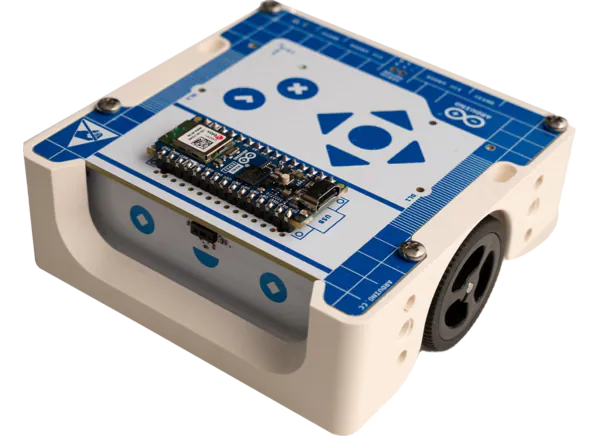
\includegraphics[width=0.6\textwidth]{Images/alvik}
  \caption{Arduino Alvik.}
  \label{fig:immagine}
\end{figure}
L'\textbf{Alvik} \cite{ArduinoAlvik} è una piattaforma robotica educativa e modulare sviluppata da \textit{Arduino},
progettato per introdurre studenti e utenti alle prime armi al mondo della robotica,
non sacrificando prestazioni e estendibilità.
\medskip

È dotato di due microcontrollori e una vasta gamma di sensori e attuatori. \\
Il microcontrollore principale è un \textit{Arduino Nano ESP32},
posizionato nella parte superiore e gestisce la logica di alto livello.
All'interno del corpo del robot, denominato \textit{carrier}, è invece integrato
un microcontrollore \textit{STM32F4}, responsabile del controllo dei sensori e attuatori. \\
L'architettura a doppio controllore permette una maggiore disponibilità di risorse per le applciazione degli utenti, i quali sono generalmente eseguiti dall'Arduino Nano.
\medskip

Il robot è dotato di un ampio set di sensori e attuatori che gli permettono di percepire l'ambiente circostante e interagire attivamente con esso.
\pagebreak
\begin{table}[h!]
\centering
\renewcommand{\arraystretch}{1.2}
\begin{tabular}{|p{4cm}|p{9cm}|}
\hline
\textbf{Microcontrollore principale} &
Arduino Nano ESP32: 
\begin{itemize}
  \item 8 MB RAM
  \item u-blox® NORA-W106 (ESP32-S3)
  \item Processore fino a 240 MHz
  \item ROM 384 kB + SRAM 512 kB
  \item 16 MB di memoria FLASH esterna
\end{itemize} \\ \hline

\textbf{Secondo microcontrollore} & STM32 Arm® Cortex®-M4 32 bit \\ \hline

\textbf{Alimentazione} & 
Nano ESP32 USB-C® con batteria Li-Ion 18650 ricaricabile e sostituibile (inclusa) \\ \hline

\textbf{Programmazione} & 
MicroPython, Arduino e programmazione a blocchi \\ \hline

\textbf{Connettività} & 
Wi-Fi®, Bluetooth® Low Energy \\ \hline

\textbf{Sensori e input} &
	Time of Flight Distance Sensor (fino a 350 cm),
	RGB Color Sensor,
	Giroscopio–accelerometro a 6 assi,
	Array line follower (x3),
	Pulsanti tattili (x7),
\\ \hline

\textbf{LED e motori} &
	2 LED RGB,
	Motori 6V – velocità a vuoto 96 rpm, corrente a vuoto 70 mA,
\\ \hline

\textbf{Estensioni} &
Connettori LEGO® Technic™ (x4),
Connettori a vite M3 (x8),
Servo motore,
I2C Grove,
I2C Qwiic,  \\ \hline
\end{tabular}
\caption{Specifiche tecniche del robot \textit{Alvik}.}
\label{tab:alvik-specs}
\end{table}

\subsection{Ambiente di sviluppo}
L'ambiente di sviluppo dell'\textit{Alvik} è \textbf{ESP-IDF}, il kit ufficiale di \textit{EspressIf} per i microcontrollori \textbf{ESP32},
a sua volta basato sul sistema operativo in tempo reale \textit{FreeRTOS}.

In tale ambiente sono disponibili una vasta e completa gamma di procedurre per la gestione di thread,
concorrenza, I/O e memoria proprie di \textit{FreeRTOS} e di \textit{ESP-IDF};
una implementazione della libreria standard \textit{C} e della \textit{STL} di \textit{C++};
varie implementazioni delle più importanti librerie usate nei sistemi \textit{UNIX} 
come \textit{pthread}, e di grandissima importanza, i \textit{Berkeley sockets}.
\medskip

Tale ricchezza ha permesso lo sviluppo di codice di alto livello \textit{portatile}, in grado
di essere facilmente utilizzato in altre piattaforme.
\medskip

Inoltre, la piattaforma \textit{Arduino}, fornisce una ulteriore astrazione a complesse operazioni,
come la configurazione di avvio del microcontrollore e la gestione del \textit{WiFi}.
\medskip

Specifica dell'\textit{Alvik} invece è la libreria per il controllo del \textit{carrier},
tale che fornisce una interfaccia a sensori e attuatori del robot, nonché servizi non banali
come odometria e stato della batteria.
\medskip



% \section{Blender}

%\begin{figure}[hb]
%  \centering
%  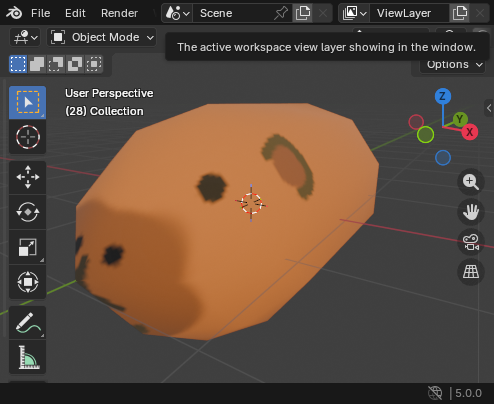
\includegraphics[width=0.5\textwidth]{Images/blender-screen.png}
%  \caption{Una schermata di Blender con assets prodotto.}
%  \label{fig:dmdte}
%\end{figure}


%Blender \cite{Blender} è un software open source e multipiattaforma per la modellazione, animazione e rendering 3D. \\
%È sviluppato e mantenuto dalla Blender Foundation ed è distribuito gratuitamente sotto licenza GPL. \\
%Il programma offre un set completo di strumenti per:
%\begin{itemize}
%	\item modellazione poligonale, NURBS e scultorea;
%	\item texturing e shading, con un potente motore di materiali basato su nodi;
%	\item animazione e rigging di personaggi;
%	\item simulazioni fisiche (fluido, fumo, tessuti, particelle);
%	\item rendering fotorealistico con i motori Cycles e Eevee;
%	\item video editing e compositing;
%	\item scripting in Python, utile per automatizzare o integrare funzionalità personalizzate.
%\end{itemize}	
%
%Grazie alla sua natura open source e all’ampia comunità di sviluppatori, Blender è oggi considerato uno degli strumenti più versatili e accessibili per la produzione 3D professionale e per l’insegnamento delle tecniche di computer grafica.
%